\cotefile{29}
\scanpage{203}
\mspage{12}
% archive sheet number: 202

\uline{reconstituer} $(R,r)$ en termes de $(C,s)$. On va montrer comment réconstituer $(R_S,r_S)$. La construction s'appliquera alors aux $R_{S'},r_{S'}$ (en travaillant sur $S'$ et appliquant ce qui \deleted{\unsure{puis|peut}} aura été fait à $R|S'$) et les foncteurs restriction seront aussi \unsure{évidents|évidentes}.

Soit $X$ un objet de $R_S$. Soit $C_X$ la sous-catégorie pleine de $C$ formée des objets $M$ \deleted{tels que}\inserted{(sur $S'\in\mathrm{Ob}\,\mathrm{Et}/S$)} \deleted{\unsure{$\varphi(M)$}}\inserted{$X_{S'}$} soit \inserted{\unsure{lui}} subordonné à \deleted{\illegible{1}}\inserted{$\varphi(M)$}. Les $S'$ correspondant à de tels $M$ \inserted{et tels que de plus $\varphi(M)\longrightarrow e_S$, soit un épim,} \uline{\unsure{recouvrent|couvrent}} $S$ par hypothèse ; \deleted{et de} \deleted{\unsure{même pour}} \unsure{dire|lieu} que $C_X$ \unsure{$\rightarrow$|est} un \uline{crible} \deleted{\unsure{couvrant}}\inserted{\uline{admissible}} de $C$. \deleted{\unsure{Soit}} Alors pour tout \deleted{tel} $M\inserted{\in\mathrm{Ob}\,C_X}$, $r(X_{S'}\times\varphi(M))\longrightarrow r\varphi(M)$ $=s(M)$ est un \deleted{morphisme}\inserted{revêtement} étale. \deleted{Donc} Ainsi $M\longmapsto r(X\times_{S'}\varphi(M))/\underset{\substack{\Vert\\s(M)}}{r(\varphi(M))}$ donne une section cartésienne de la catégorie fibrée sur $C_X$ induite par \deleted{\unsure{la ss Cat|la source}} $\mathrm{EtFl}_S$ (catégorie fibrée \inserted{sur $\mathrm{Fl}_S$} des revêtements étales relatifs) via $C_X\xrightarrow{s}\mathrm{Fl}_S$. \deleted{\unsure{On trouve}} Soit $\unsure{\mathcal E|E}$ la catégorie fibrée obtenue \inserted{ainsi} sur $C$ via $s:C\longrightarrow\mathrm{Fl}_S$, \deleted{\unsure{on trouve}} Si $C_0$ est n'importe quel crible de $C_{\deleted{\unsure{X|0}}}$, \deleted{\unsure{on trouve}} \unsure{soit} $R_S^{C_0}$ \deleted{un fonct} la sous-catégorie \deleted{fibrée} de $R_S$ formée des objets $X\deleted{\unsure{_{S'}}}$ tels que $\forall\,S'\in\mathrm{Ob}\,\mathrm{Et}(S)$, \deleted{\unsure{$X_{S'}$ est sub}} $X_{S'}$ est \deleted{\unsure{donc|loc.}} subordonné à tt objet de $C_0$ sur $S'$. On trouve donc une ss-catégorie multigaloisienne de $R_S^{\unsure{C}}$, stable par $\mathop{\underleftarrow{\mathrm{Lim}}}\limits$ et \deleted{\unsure{fonct}} \unsure{sommands|sommes} directs et un foncteur

\[
\alpha:R_S^{C_0}\longrightarrow\mathop{\underleftarrow{\mathrm{Lim}}}\limits_{C_0}(\mathcal E|C_0)
\tag*{$(*)$}
\]

\scanpage{204}
\mspage{13}
% archive sheet number: 203

Pour $C_0$ parcourant les cribles \deleted{\uline{couvrants}}\inserted{admissibles} de $C$, \deleted{les $R$} et admettant que la catégorie \inserted{fibrée} \uline{$C$ est loc\textsuperscript{t}} \uline{filtrante}, ce qui implique que l'intersection de deux cribles couvrants est encore couvrant, on voit que les $R_S^{C_0}$ forment une famille filtrante de ss-catégories multigaloisiennes pleines de $R_S$, de réunion $R_S$. Donc on gagne si on sait que les foncteurs $\alpha$ sont des \uline{équivalences} de catégories, car on aura alors une équivalence

\[
R_S\approxeq\mathop{\underrightarrow{\mathrm{Lim}}}\limits_{\substack{C_0\\\text{variable}}}\ \mathop{\underleftarrow{\mathrm{Lim}}}\limits_{\text{sur }C_0}(\unsure{\mathcal E|E}|C_0)
\]

qui \unsure{explicitent|explicite} $R_S$ en termes de $(C,s)$, \unsure{sous réserve|pourvu vérifiée|qui reste} tout au moins que la notion de \uline{crible admissible}

% margin note written sideways
\margin{soit connue. Il en sera ainsi si on impose que pour tt $M\in\mathrm{Ob}\,C_{S'}$, $(S'\in\mathrm{Ob}\,\mathrm{Et}(S))$ $\varphi(M)\longrightarrow e_{S'}$ \uline{est épimorphisme dans $R_{S'}$} ; \uline{c'est ce que nous supposerons par la suite} pour simplifier (Mais ce n'est pas très naturel pour les \unsure{mouvements|monuments} \unsure{alg.} ! On en doit \unsure{pouvoir} \unsure{justifier|particulariser} \unsure{G.R.} !)}

On va montrer que pour que $\alpha$ soit une équivalence (pour $C_0$ crible couvrant) il suffit que $\varphi$ soit \uline{pleinement fidèle}.

\margin{\unsure{Supposons|Supposant} \unsure{tjs} $C$ loc. filtrante}

Comme $\alpha$ est un foncteur exact de catégories multigaloisiennes, il suffit de voir pour la \deleted{\unsure{plei|plus}}fidélité que $\alpha(X)=\emptyset\Longrightarrow X=\emptyset$, ce qui est immédiat grâce au fait $C_0$ \deleted{couvrant}\inserted{admissible} : c'est local pour (Et), on peut supposer donc qu'il existe un $M\in C_{0S}$, \inserted{avec $\varphi(M)\longrightarrow e_S$ épim,} alors comme $r(\varphi(M)\times X)=\emptyset$ on a $\varphi(M)\times X=\emptyset$, OK.

$\alpha$ pleinement fidèle ? Soit $X\in\mathrm{Ob}\,R_S^{C_0}$, et $Z=\alpha(X)=Z_1\amalg Z_2$, montrer que cette

\scanpage{205}
\mspage{14}
% archive sheet number: 204

décomposition est induite par une décomposition de $X$. La question étant locale sur $S$, on peut supposer $\exists\,M\in\mathrm{Ob}\,C_S$, $\varphi(M)\longrightarrow e$ un épimorphisme.

Considérons $r(X\times\varphi(M))=\alpha(X)(M)\inserted{=Z(M)}\longrightarrow r\varphi(M)=s(M)$ il se coupe en $Z_1(M)\amalg Z_2(M)$, donc \deleted{par} R2 $X\times\varphi(M)$ se coupe en $X_1\amalg X_2$. Je dis que

\diagram{\begin{tikzcd}[ampersand replacement=\&,column sep=small,row sep=small]
T\arrow[d,shift left=.5ex]\arrow[d,shift right=.5ex]\&X\times T\arrow[d,shift left=.5ex]\arrow[d,shift right=.5ex]\&\\
\varphi(M)\arrow[d]\&X\times\varphi(M)\arrow[l,dash]\arrow[d]\&X_1\arrow[l,hook]\\
e\&X\arrow[l,dash]\&
\end{tikzcd}}

cette décomposition provient d'une décomposition de $X$, i.e. que quels que soient \deleted{\unsure{du|les}} l'objet \deleted{\unsure{Z|T}}\inserted{$T$} de $R_S^{C_0}$ et deux morphismes $T\rightrightarrows\varphi(M)$, les deux images inverses de $X_1$ par $T\rightrightarrows\varphi(M)$ sont les \unsure{mêmes}, ou

% slanted
\margin{\unsure{encore dont|encore deux|encore dans|on a} les $\leftleftarrows$ \unsure{sont} \deleted{\unsure{égaux}} $r(X_1)\rightrightarrows r(X\times T)$}

Or, \inserted{quitte à ajouter à $T$ un objet $\varphi(M)$ (qui envoie deux fois dans $\varphi(M)$ par id) on peut supposer} \deleted{quitte à localiser $T$ lui est subordonné à} \deleted{$\varphi(M)$, ce qui implique} $T\longrightarrow e_S$ épim., donc $T\times\varphi(M)\longrightarrow\varphi(M)$ un épim. Comme $T\deleted{\times\varphi(M)}$ est subordonné à $\varphi(M)$,

$T\times\varphi(M)$ est constant par morceaux sur $\varphi(M)$, et étant épimorphique, \unsure{cela|il} est \uline{recouvert} (pour sa topologie canonique, p. ex.) par les images des sections $w$ de \deleted{\unsure{$\varphi$}} $T\times\varphi(M)$ sur $\varphi(M)$, Ceci posé, on peut remplacer $T\rightrightarrows\varphi(M)$ par les composés $T\times\varphi(M)\xrightarrow{\mathrm{pr}_1}T\rightrightarrows\varphi(M)$ (car $\mathrm{pr}_1$ est épim., $\varphi(M)\longrightarrow e_S$ l'étant !), puis \unsure{ces derniers|ce dernier|en dernier} par les composés $\varphi(M)\xrightarrow{w}T\times\varphi(M)$. Bref, on est ramené au cas où $T=\varphi(M)$. Mais $\varphi$ étant pl. fidèle

\scanpage{206}
\mspage{15}
% archive sheet number: 205

on trouve que les deux flèches sont induites par $M\rightrightarrows M$, et \unsure{on|\deleted{on}} \deleted{gagne} trouve que les deux images de $r(X_1)$ \unsure{au|en|dans} $r(X\times T)=r(X\times\varphi(M))$ $=\deleted{\unsure{\alpha}}\alpha(X)(M)$ est $Z_1(M)$.

On a donc trouvé une décomposition $X=X_1\amalg X_2$, \deleted{tq dès que $Z_1=\alpha(X_1)$} \inserted{uniqt déterminée par la condition que} la décomposition correspondante de $\alpha(X)(M)$ est donnée par \deleted{i.e. que pour tt $M'$ sur un} $Z_1(M)$. \deleted{Si on a}

\deleted{un autre $M'$, et si} \deleted{est le ``complément''} \deleted{Considérons en effet $Z'_1=\alpha(X_1)$, pq dès lors} \deleted{\inserted{de} $Z_1\cap Z'_1$ dans $Z_1$ et $Z'_1$, soient $A$ et $B$. On a} \deleted{\unsure{donc} $A(M)=\emptyset$, $B(M)=\emptyset$, \deleted{on prouvera que} \inserted{prouvons $A=\emptyset$, $B=\emptyset$}} \deleted{i.e. pour tt $M'\in C_{0S'}$, \inserted{$A(M')=\emptyset$, $B(M')=\emptyset$}} \deleted{pour un objet \unsure{$A$} de \unsure{$R$} \unsure{ou} $\unsure{\mathcal E|E}|C_0$,}

\deleted{$A(M)=\emptyset\Longrightarrow M=\emptyset$. En effet, soit $M'\in C_0$ sur $S'$,}
\deleted{prouvons $A(M')=\emptyset$. \uline{\unsure{Quitte|Celà|à vérifier} à se restreindre} à $S'$, on}
% slanted
\margin{\unsure{expliciter}\ldots}
\deleted{peut supposer $S'=S$, et Si on a un morphisme}
\deleted{\unsure{Alors} \unsure{on a} $A(M\times M')=\emptyset$, donc}

\deleted{or $A(M\times M')=A(M')\times_{s(M')}s(M\times M')$, il} \deleted{suffit donc de voir que $s(M\times M')\longrightarrow s(M')$} \deleted{est \uline{surjectif} ou encore} \deleted{$r(\varphi(M\unsure{\times}$} \deleted{$M'\longrightarrow M$, c'est trivial. Sinon,} \deleted{quitte à se localiser, il existe}

\diagram{\begin{tikzcd}[ampersand replacement=\&,row sep=small,column sep=small]
\&\deleted{\varphi(M)\times\varphi M'}\arrow[dl]\arrow[dr]\&\\
\deleted{\varphi(M)}\&\&\deleted{\varphi(M')}
\end{tikzcd}}

\diagram{\begin{tikzcd}[ampersand replacement=\&,row sep=small,column sep=small]
\&\deleted{M''}\arrow[dl]\arrow[dr]\&\\
\deleted{M}\&\&\deleted{M'}.
\end{tikzcd}}

\deleted{Alors $A(M'')=\emptyset$, $B(M'')=\emptyset$. Donc la décomposition} \deleted{$X=X_1\amalg X_2$ est aussi celle qui serait définie} \deleted{en prenant $M''$, au lieu de $M$. \unsure{Mais} il y en} \deleted{a une aussi avec $M'$, soit $X=X'_1\amalg X'_2$,} \deleted{et c'est aussi celle}

\scanpage{207}
\mspage{16}
% archive sheet number: 206

un autre $M'$, et si $\unsure{\exists|{\rlap{\text{!}}\exists}|\nexists}\,M'\longrightarrow M$, \deleted{alors} il est évident que la décomposition de \unsure{$X$|\deleted{$X$}} définie par $M'$ est la \unsure{m.} Localisant sur $S$ et utilisant le fait que $C$ est loc. filtrante, on trouve que la décomposition ne dépend pas du choix de $M$. Localisant à nouveau sur $S$, on voit qu'elle définit la décomposition donnée de $Z$\unsure{.|:}

Prouvons que $\alpha$ est \uline{essentiellement} \uline{surjectif}.

\scanpage{209}
\mspage{1}
% archive sheet number: 208

\uline{Catégories multigaloisiennes.}

$\mathcal U$ un univers

$C$ une catégorie

A) \uline{Conditions équivalentes}

(i) Il existe un $\mathcal U$-topos $\mathscr T$, et une équivalence

\[
C\approxeq\mathscr T_{\deleted{\unsure{\mathrm{lcf}}}\unsure{\mathrm{revf}|\mathrm{rev}\,f|\mathrm{cf}}}
\]

où $\mathscr T_{\mathrm{revf}}$ est la \unsure{ss-catégorie|catégorie} pleine de $\mathscr T$ formée des objets loc\textsuperscript{t} ``constants finis''.

(ii) \inserted{$C$ est une $\mathcal U$-catégorie, l'ens des objets mod isom \inserted{de $C$} est $\mathcal U$-petit, et} Il existe une topologie sur $C$, [moins fine que la canonique,] et telle que le foncteur can $C\longrightarrow\widetilde C$ induise une équivalence $C\longrightarrow\widetilde C_{\mathrm{revf}}$.

(ii bis) Itou, en prenant la ``topologie de la descente effective universelle''.

(iii) \inserted{$C$ est une $\mathcal U$-catégorie, dont l'ens des objets mod iso. est $\mathcal U$-petit ;} Pour tout objet $X$ de $C$, \deleted{l'\unsure{ensemble|ens. des|ensemble des}} objets $S$ tels que $X_S$ sur $S$ soit constant fini sur $S$ forment une famille \deleted{couvrante} de descente effective universelle.

(iv) Cf conditions sur feuille 1 bis

B) \uline{Conditions équivalentes}

\deleted{(i) Comme (i) dessus, mais en exigeant de plus} \deleted{que l'objet final de $\mathscr T$ est somme \uline{finie} d'objets} \deleted{connexes}

\deleted{(ii) (ii bis) (iii) Comme plus haut, mais en} \deleted{exigeant que l'objet final de $C$ (ou encore,} \deleted{tout objet de $C$, au choix) est somme finie} \deleted{d'objets connexes.}

\deleted{(iv) $C$ satisfait aux conditions suivantes.}

(i) $C$ satisfait aux conditions de A), et son objet final est somme effective universelle d'objets connexes.

\scanpage{210}
\mspage{2}
% archive sheet number: 209

(ii) On a les conditions G0 à G5

G0 $C$ est une $\mathcal U$-catégorie, l'ens des \deleted{\unsure{classes mod}} isomorphies d'objets de $C$ est $\mathcal U$-petit

G1 Existence de $\underleftarrow{\mathrm{Lim}}$ \inserted{finies} et \deleted{$\underrightarrow{\mathrm{Lim}}$}\inserted{sommes} \uline{finies}

G2 \deleted{Les \unsure{équi|épim.}relations d'équivalence sont effectives,} \deleted{les épimorphismes sont effectifs universels,} les sommes finies \deleted{sont} disjointes \deleted{\unsure{eff|effect|épi.}}\unsure{universelles|effectives}.

G3 Tout morphisme $X\longrightarrow Y$ se factorise en \deleted{épimorphisme}\inserted{morphisme de descente effective} suivi de isom. sur sommand direct.

G4 \deleted{Tout} L'objet \inserted{final} est \deleted{\unsure{localt|une} (ou au choix, \unsure{arbitraire})} somme \deleted{\unsure{disjoint|disjointe}} effective univ. d'objets connexes.

G5 \deleted{pour les \unsure{sous-objets|sous - objets} [ou encore : l'objet final est} \deleted{somme \uline{finie} d'objets connexes].} soit $d:X\longrightarrow Y$ avec $X,Y$ connexes, alors $\exists$ entier $N$ tel que pour tt $Y'\longrightarrow Y$, $Y'\ne\emptyset_C$, \deleted{\unsure{l'élément}} $X\times_Y Y'$ ne contient pas $Y'\times\unsure{[1,N+1]|[1,N+1[}$ \inserted{comme sommand}.

(\deleted{\unsure{vi}}\inserted{iii}) \deleted{Il existe} $C$ est équivalente à une catégorie produit \deleted{\illegible{1}} $\prod_{i\in I}C_i$, les $C_i$ \uline{galoisiennes}.

[NB les $C_i$ correspondent donc aux composantes connexes \inserted{$e_i$} de l'objet final ; la donnée d'une équivalence $C_i\simeq C(\pi_i)$ correspond à la donnée d'un foncteur fibre \inserted{de $C/e_i$}, ou d'un ``rev. universel'' de l'objet \deleted{\unsure{$f$}} $e_i$].

\uline{Démonstration de A}

$(\mathrm{iii})\Longrightarrow(\mathrm{ii\ bis})\Longrightarrow(\mathrm{ii})\Longrightarrow(\mathrm{i})$ triviaux, et $(\mathrm{i})\Longrightarrow(\mathrm{iii})$ aussi, car si $X\in\mathscr T_{\unsure{\mathrm{revf}|\mathrm{rev}\,f|\mathrm{cf}}}$, alors l'objet final $e$ de $\mathscr T$ est somme (dans $\mathscr T$) d'objets $e_i$ $(i\in\mathbb N)$ avec $X|e_i$ de rang $i$. De plus, $\underline{\mathrm{Isom}}_{e_i}([1,i]_{e_i},X)=P_i$ est alors un objet de $\mathscr T_{\mathrm{revf}}$ tel que $\unsure{P|R}_i\longrightarrow e_i$ épim (c'est un torseur sous $(\mathfrak S_i)_{e_i}$ !) et tel que

\scanpage{211}
\mspage{3}
% archive sheet number: 210

$X_{P_i}\simeq[1,i]_{P_i}$. Les $P_i\longrightarrow e$ forment une famille \deleted{épimorphique} de descente effective universelle \deleted{pour} dans $\mathscr T$, donc aussi dans $\mathscr T_{\unsure{\mathrm{revf}|\mathrm{rev}\,f|\mathrm{cf}}}$ (N.B. $\mathscr T_{\mathrm{revf}}$ \deleted{\unsure{admet des|stable}}\inserted{est stable} par produits finis -- en fait par $\underleftarrow{\lim}$ et $\underrightarrow{\lim}$ \uline{finis}).

\uline{Démonstration de B}

\deleted{En fait, on constate aisément que} \deleted{les conditions de A(i) impliquent G0 G1 G2 G3.}

\deleted{L'équivalence de (i) \unsure{:|à|et} (iii) tient au fait que} \deleted{les décompositions en sommes de $e$, dans $\mathscr T_{\mathrm{revf}}$} \deleted{ou dans $\mathscr T$, sont les \unsure{m\textsuperscript{es}} ; donc dire que $e$} \deleted{est somme finie d'objets connexes dans $\mathscr T$, ou} \deleted{dans $C$, revient au \unsure{m\textsuperscript{e}}.}

\deleted{Pour prouver que ces conditions impliquent (iv)} \deleted{il \deleted{faut}\inserted{reste à} prouver \deleted{que} qu'elles impliquent G4,} \deleted{i.e. tout revêtement fini d'un objet connexe $e$} \deleted{est somme finie d'objet connexes. En fait,} \deleted{si $X$ est de rang $n$ sur $e$, on trouve que} \deleted{le nb de composantes connexes de $X$ est $\le n$,} \deleted{et égal à $n$ ssi $X$ est trivial : c'est immédiat} \deleted{par récurrence sur $n$, et additivité du rang.}

\deleted{$(\mathrm{v})\Longrightarrow(\mathrm{iii})$ est immédiat ; on prend pour $\mathscr T$ le topos} \deleted{``somme'' des $B_{\pi_i}$. ($B_{\pi_i}=$ ensembles discrets sur} \deleted{lequel $\pi$ opère continûment).}

Il resterait à prouver $(\mathrm{ii})\Longrightarrow(\mathrm{iii})$. Je préfère prouver d'abord $(\mathrm{ii})\Longrightarrow(\unsure{\mathrm{i}|\mathrm{ii}|\mathrm{iii}}\deleted{\unsure{v}})$.

\scanpage{212}
\mspage{4}
% archive sheet number: 211

\unsure{Donc|Pour} moyennant G0 à G4, il faut prouver ceci : si $X\in\mathrm{Ob}\,C$, alors il \deleted{existe famille de descente effective} \deleted{universelle}\inserted{les} $S_i\longrightarrow e$, \unsure{tels|telles} que les $X_{S_i}/S_i$ soient constants finis, recouvrent $e$ pour la topologie de la descente effective. Utilisant G2 et G4, on est

\deleted{Soit $e_i$ \unsure{distincts} de $e$, \deleted{\unsure{donné}}\inserted{sommand} direct de $e$} \deleted{[G3] \deleted{et G2, entrainent que un \unsure{isomorphisme} d'un} prenons les parties finies $J$ de $I$, on peut} \deleted{\deleted{\unsure{monomorphisme direct}} considérer \deleted{$\unsure{\pi_J}$} $\operatorname{Sup}_{i\in J}e_i$ (sommes sont disjointes} \deleted{et universelles, et produits fibrés existent), ils} \deleted{forment une famille croissante d'objets, donc stationnaire.} \deleted{Soit $e'$ la valeur stationnaire, et $e''$ son ``complémentaire''.} \deleted{Je dis que $e''=\emptyset$ i.e. $e'=e$.} \deleted{En effet, considérons $X_{e''}$ sur $e''$, alors}

ramené à prouver que si $X\longrightarrow Y$ ($Y$ sommand direct de $e$, mais peu importe) est tel que $Y$ connexe $\ne\emptyset$, \unsure{et} $X$ connexe, alors $\exists\,Y'\longrightarrow Y$ de descente eff. universelle, avec $X_{Y'}\simeq[1,n]_{Y'}$ ($n$ convenable). On \deleted{\unsure{regarde la démarche|en baissant les dimensions}}\inserted{procède par récurrence sur l'entier} \deleted{\unsure{N}} $n$ de G5 (majorant le rang], en reprenant la démonstration plus haut

\uline{Remarque} : il se pourrait que G5 soit surabondant.

Noter qu'en présence des autres axiomes, on peut le remplacer par :

G5$'$ \deleted{\unsure{Il ex}} Pour tt composante connexe $e_i$ de $e$, $\exists$ foncteur exact $F:C\longrightarrow(\mathrm{Ens}\,f]$ tel que $F(e_i)\unsure{\ne|=}\emptyset$

\scanpage{213}
\mspage{1 bis}
% archive sheet number: 212

\deleted{$\exists$ fonction}

\textcircled{3} On peut trouver, pour tt $n\in\mathbb N$, la classe des ``morphismes de degré $n$'', de façon que

\uline{a)} Stabilité par changt de base

\uline{b)} additivité finie

\uline{c)} Un isom. est de degré 1

\uline{f)} Si $f:X\longrightarrow Y$, alors $Y=\coprod_{n\in\mathbb N}Y_n$, somme directe disjointe, effective, universelle, tels que $X_n=X\times_Y Y_n\longrightarrow Y_n$ soit de degré $n$.

\uline{d)} Si $f:X\longrightarrow Y$ est de degré $n\ge1$, alors $f$ est un morphisme de descente effective [donc de descente effective \uline{universelle} grâce à a)]

\uline{e)} Si $f:X\longrightarrow Y$ est de degré 0, alors $X=\emptyset_C$

\textcircled{2} Tout monomorphisme est un isomorphisme avec un sommand direct universel

\textcircled{1} Existence de $\underleftarrow{\mathrm{lim}}$ finies

\deleted{\textcircled{\unsure{1|0}}} \unsure{$e$|\deleted{$e$}}

\textcircled{0} $C$ est une $\mathcal U$-catégorie (i.e. les $\mathrm{Hom}(X,Y)$ sont $\mathcal U$-petits) et l'ens des classes d'isom. d'objets de $C$ est $\mathcal U$-petit.

\unsure{'} Implique condition A(iii). En effet, à prouver que pour $X$ donné, les $S\longrightarrow e$ tels que $X_S$ constant fini sur $S$ font famille \unsure{de|de la} descente eff. universelle. Grâce à 3 f), on est ramené à prouver l'analogue pour $X\longrightarrow Y$ au lieu de $X\longrightarrow e$, mais avec $X\longrightarrow Y$ de degré $n$. \inserted{à trouver un morphisme de \unsure{desc. eff. univ.|descente eff. universelle} \deleted{\unsure{ou}} qui trivialise $X$} \inserted{Si} $n=0$, on conclut par 3 e que $X=\emptyset$, on prend $Y\longrightarrow Y$ ($X=\unsure{\emptyset_{/Y}|\emptyset_Y}$ !). Si $n>0$, on procède par récurrence, supposant que

\scanpage{214}
% archive sheet number: 213

\diagram{\begin{tikzcd}[ampersand replacement=\&,column sep=large,row sep=small]
\deleted{X^P}\arrow[r,hook,"\deleted{\alpha_P}","{\text{\deleted{imm. fermée}}}"']\arrow[d]\&\deleted{X^E}\\
\deleted{F_P}\&
\end{tikzcd}}

\[
\deleted{X^E=\bigcup_{\substack{P\\\text{(disjointe)}}}\alpha_P((X^P)^*)}
\]

\[
\deleted{(f^E)^{-1}(\Delta_Y^{(E)})=\bigcup_{\substack{P\\\text{somme}\\\text{disjointe}}}
\underbrace{\alpha_P(F_P)}_{\substack{\text{de dim }n-(\operatorname{card}P-1)d\,\geq\,n-\operatorname{card}(E)d\\
\text{égalité pour }P=\underbrace{P_0}_{\text{partition maximale}}\text{ seulement}}}}
\]

\[
\begin{aligned}
&\deleted{\underline{\operatorname{Card}} E=3} &\deleted{\text{partition en }3:P_0}\\
&&\deleted{\text{partitions en }2:(1)(23),(2)(31),(3)(12)}\quad\deleted{P_{23}\quad P_{31}\quad P_{12}}\\
&&\deleted{\text{partition en }3:P_1}
\end{aligned}
\]

\[
\deleted{(f^3)^{-1}(\Delta_Y^{(3)})=
\underset{n-2d}{F_3}\ \cup\!
\bigcup_{1\leq i<j\leq 3}\underset{n-d}{\alpha_{ij}(F_2)}\ \cup\
\underset{n}{\Delta_X^{(3)}}}
\]

\deleted{dim ``génériques''}

\deleted{\uline{Question}}

\[
\begin{aligned}
&\deleted{\overline F_3\cap\Delta_X^{(3)}=\emptyset}\\
&\deleted{\overline{\alpha_{ij}(F_2)}\cap\Delta_X^3=\alpha_{ij}(\overline F_2)\cap\Delta_X^{(3)}
=\alpha_{ij}(\underbrace{\overline F_2\cap\Delta_X^{(3)}}_{\substack{=\emptyset\ \text{si}\\f\ \text{\unsure{net}}}})=\boxed{\emptyset}}\\
&\deleted{\overline F_3\cap\overline{\alpha_{ij}(F_2)}\unsure{\mathord{\cdot}|=|,}\overline F_3\cap\alpha_{ij}(\overline F_2)}
\end{aligned}
\]

\deleted{\uline{NB} Si $f$ net, alors $\overline F_3\cap\underset{\text{fermé}}{\Delta_X^{(3)}}=\emptyset$, $\overline{\alpha_{ij}(F_{\unsure{1|2}})}\cap\Delta_X^{(3)}=\emptyset$}

\deleted{Mais que peut-on dire de}

\[
\deleted{\overline F_3\cap\overline{\alpha_{ij}(F_2)}\mathord{\cdot}\overline F_3\cap\alpha_{ij}(\overline F_2)}
\]

\[
\deleted{\underbrace{x_1^{\unsure{\lambda|d|0}}\ne x_2^\lambda\ne x_3^\lambda}_{\ne}}
\qquad \underbrace{x_1^0=x_3^0}\ne x_2^0
\]

\figure{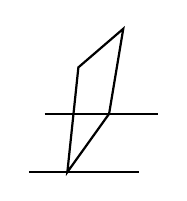
\begin{tikzpicture}[x=1cm,y=1cm,line width=.8pt]
\draw (-.2,0)--(1.2,0); \draw (0,.74)--(1.44,.74);
\draw (.29,0)--(.43,1.33)--(1,1.82)--(.82,.74)--cycle;
\end{tikzpicture}}

\figure{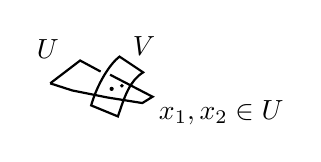
\begin{tikzpicture}[x=1cm,y=1cm,line width=.8pt]
\draw (0,.55)--(.38,.84)--(.64,.70) (.76,.66)--(1.3,.38)--(1.17,.30)--(.73,.37)--(.28,.46)--(0,.55);
\draw (.52,.27) .. controls (.60,.55) and (.76,.80) .. (.88,.89)--(1.18,.69) .. controls (1.01,.58) and (.95,.40) .. (.86,.13)--cycle;
\fill (.78,.48) circle (.027); \fill (.91,.52) circle (.025);
\node at (-.03,.98) {$U$};\node at (1.19,1.02) {$V$};\node[anchor=west] at (1.25,.18) {$x_1,x_2\in U$};
\end{tikzpicture}}

\diagram{\begin{tikzcd}[ampersand replacement=\&,row sep=small,column sep=small]
X(1)\arrow[dr,bend right=12]\&\&X(2)\arrow[dl,bend left=12]\\
\&Y\&
\end{tikzcd}}

\[
\begin{aligned}
&\dim X=3\quad\dim Y=4\\
&\dim F_3=1\\
&\dim\alpha_{ij}(\overline F_{\unsure{2|1}})=2
\end{aligned}
\]

\scanpage{215}
\mspage{1 ter}
% archive sheet number: 214

c'est prouvé pour les entiers $<n$. \{ Utilisons 3 \unsure{d},

\diagram{\begin{tikzcd}[ampersand replacement=\&,row sep=small,column sep=small]
X\arrow[d]\&X\times_Y X=X'\arrow[l]\arrow[d]\\
Y\&X=Y'\arrow[l,dash]
\end{tikzcd}}

et \unsure{regarder|regardons} le \deleted{\unsure{quotient|épimorphisme}}\inserted{morphisme} \unsure{diagonale|diagonal} $\Delta_{X/Y}$, \deleted{\unsure{par 2}} (existe par \textcircled{1}), par \textcircled{2} c'est un isom avec un sommand direct \inserted{universel}, donc $X'\simeq Y'\amalg X'_1$ ; par 3 a) $X'\longrightarrow Y'$

est de degré \unsure{$n$|$n-1$}, \deleted{\unsure{de}} par 3 \uline{c} $Y'\longrightarrow Y'$ est de degré 1, donc par 3 \uline{b} et \uline{f} on voit que $X'_1\longrightarrow Y'$ est de degré $n-1$. Lui appliquant l'hyp. de récurrence, on trouve $Y''_{\unsure{i|j|s}}\longrightarrow Y'$ \deleted{famille} de descente eff. universelle, qui trivialise $X'_1$ ; comme $X'\simeq Y'\amalg X'_1$ \uline{universellt},

on a $X''=X\times_Y Y''\simeq Y''\amalg\underbrace{(X'_1\times_{Y'}Y'')}_{Y''\times[1,n-1]}=Y''\times[1,n]$. Or $Y''\longrightarrow Y$ est de descente effective universelle, comme composé de deux tels, OK.

\uline{Explicitation} Pour vérifier qu'un \deleted{$f$} morphisme est de descente effective [cf condition 3 a)], il suffit de savoir que c'est un épimorphisme effectif universel, et de savoir que les relations d'équivalence sont effectives universelles \texttt{------}

\diagram{\begin{tikzcd}[ampersand replacement=\&,row sep=small,column sep=small]
{\tikz[baseline=-.3ex]{\draw[densely dotted,line width=.7pt] (0,.2)--(.17,.2)--(0,0)--(.17,0);}}\arrow[d]\&Z_X\arrow[l,dashed]\arrow[d]\&D\arrow[l,shift left=.5ex]\arrow[l,shift right=.5ex]\arrow[d]\\
Y\&X\arrow[l]\&X\times_Y X\arrow[l,shift left=.5ex]\arrow[l,shift right=.5ex]
\end{tikzcd}}

\noindent\rule{.25\linewidth}{.3pt}

\uline{Corollaire} Sous les conditions de A (iv), la notion de ``morphisme de degré $n$'' est uniquement déterminée, et \deleted{\unsure{corresp|correspond}} équivaut à : $\exists\,Y'\longrightarrow Y$ épimorphisme (\unsure{néces.} \deleted{\unsure{morphe}} effectif universel, i.e. de descente effec\ldots{}) avec $X\times_Y Y'\simeq[1,n]_{Y'}$ ($Y'$-isom).

\scanpage{216}
\mspage{5}
% archive sheet number: [2]15

C. \uline{Corollaire} Conditions équivalentes

(i) Comme A (i), avec l'objet final de $\mathscr T$ connexe

(ii) (ii bis) (iii) (iv) Comme dans A, en supposant de plus l'objet final de de $C$ connexe

(\unsure{v|iv}) \unsure{On a|Comme} \deleted{\unsure{de|A(iv)}} les axiomes G0 G1 G2 G3, et de plus : $\exists$ foncteur \deleted{\uline{\unsure{exact cons|conservatif}}}

\[
F:C\longrightarrow(\mathrm{Ens\ finis})
\]

qui est conservatif, exact à gauche et commute aux sommes finies.

(vi) Il existe un gpe profini $\pi$ et une équivalence $C\approxeqC(\pi)$.

\scanpage{217}
\mspage{6}
% archive sheet number: 216

\uline{Proposition} Soit $u:C\longrightarrow C'$ un foncteur exact, avec $C,C'$ des catégories multigaloisiennes. Alors :

(i) $u$ fidèle $\Longleftrightarrow$ $u$ conservatif $\Longleftrightarrow$ pour tt objet $X$ de $C$, $u(X)=\emptyset\Longrightarrow X=\emptyset$

(ii) $u$ pleinement fidèle $\Longleftrightarrow$ pour tt objet $X$ de $C$, \deleted{tout} l'application $\unsure{Y|Y'}\mapsto u(\unsure{Y|Y'|X})\unsure{'|,}$ est une bijection de l'ens des sous-objets de $X$ \deleted{avec}\unsure{à|avec} l'ens des ss-objets de $Y$.

% slanted
\margin{$\longleftrightarrow$ si $u$ est pl. fidèle, alors \deleted{\unsure{sa classe}}\inserted{l'image \unsure{essentielle}} est stable par \unsure{sous-objet|ss-objet|ss.-objets} et \deleted{\unsure{images}} par objet subordonnés.}

(iii) $u$ une équivalence $\Longleftrightarrow$ $u$ est pl. fidèle (cf \unsure{(i)|(ii)}) et tout objet de $C'$ est subordonné à un objet de la forme $u(X)$ \ldots.

